As mentioned in Section~\ref{subsec:userinterface} Google Glass is equipped with a camera that could be used to take photos from the user's perspective. One potential use of the camera would be to scan Quick Response (QR) codes. The QR Code was announced in 1994. Having been under development for several years at Denso Wave~\cite{qrCodeHistory} the goal was to create a new form of barcode that could carry more information than a linear barcode and be easily read.

A conventional barcode is capable of storing approximately 20 digits while a QR code can store several thousand digits~\cite{qrCodeType}. Information is encoded using standardised encoding modes and displayed as a 2D barcode. A QR code has several standardised fields, as seen in Figure~\ref{qrcodeMall}. Using position fields a QR code can be read from any direction, compared to a conventional barcode which can only be read horizontally~\cite{qrCodeAbout}.

%	\begin{figure}[H]%ht!]
%		\centering
%		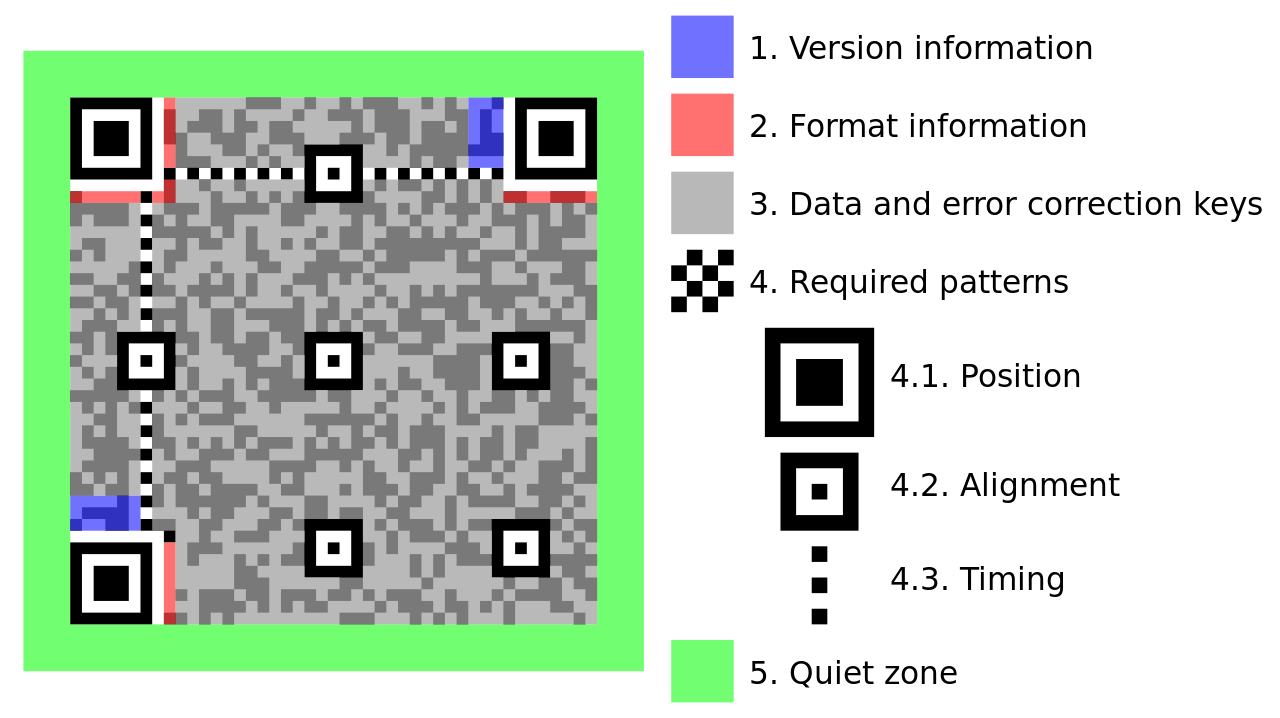
\includegraphics[width=110mm]{images/qrcodestandard}
%		\caption{The standardised fields in a QR Code~\cite{qrCodeWiki}.}
%		\label{qrcodestandard}
%	\end{figure}
	
	\begin{figure}[H]%ht!]
		\centering
		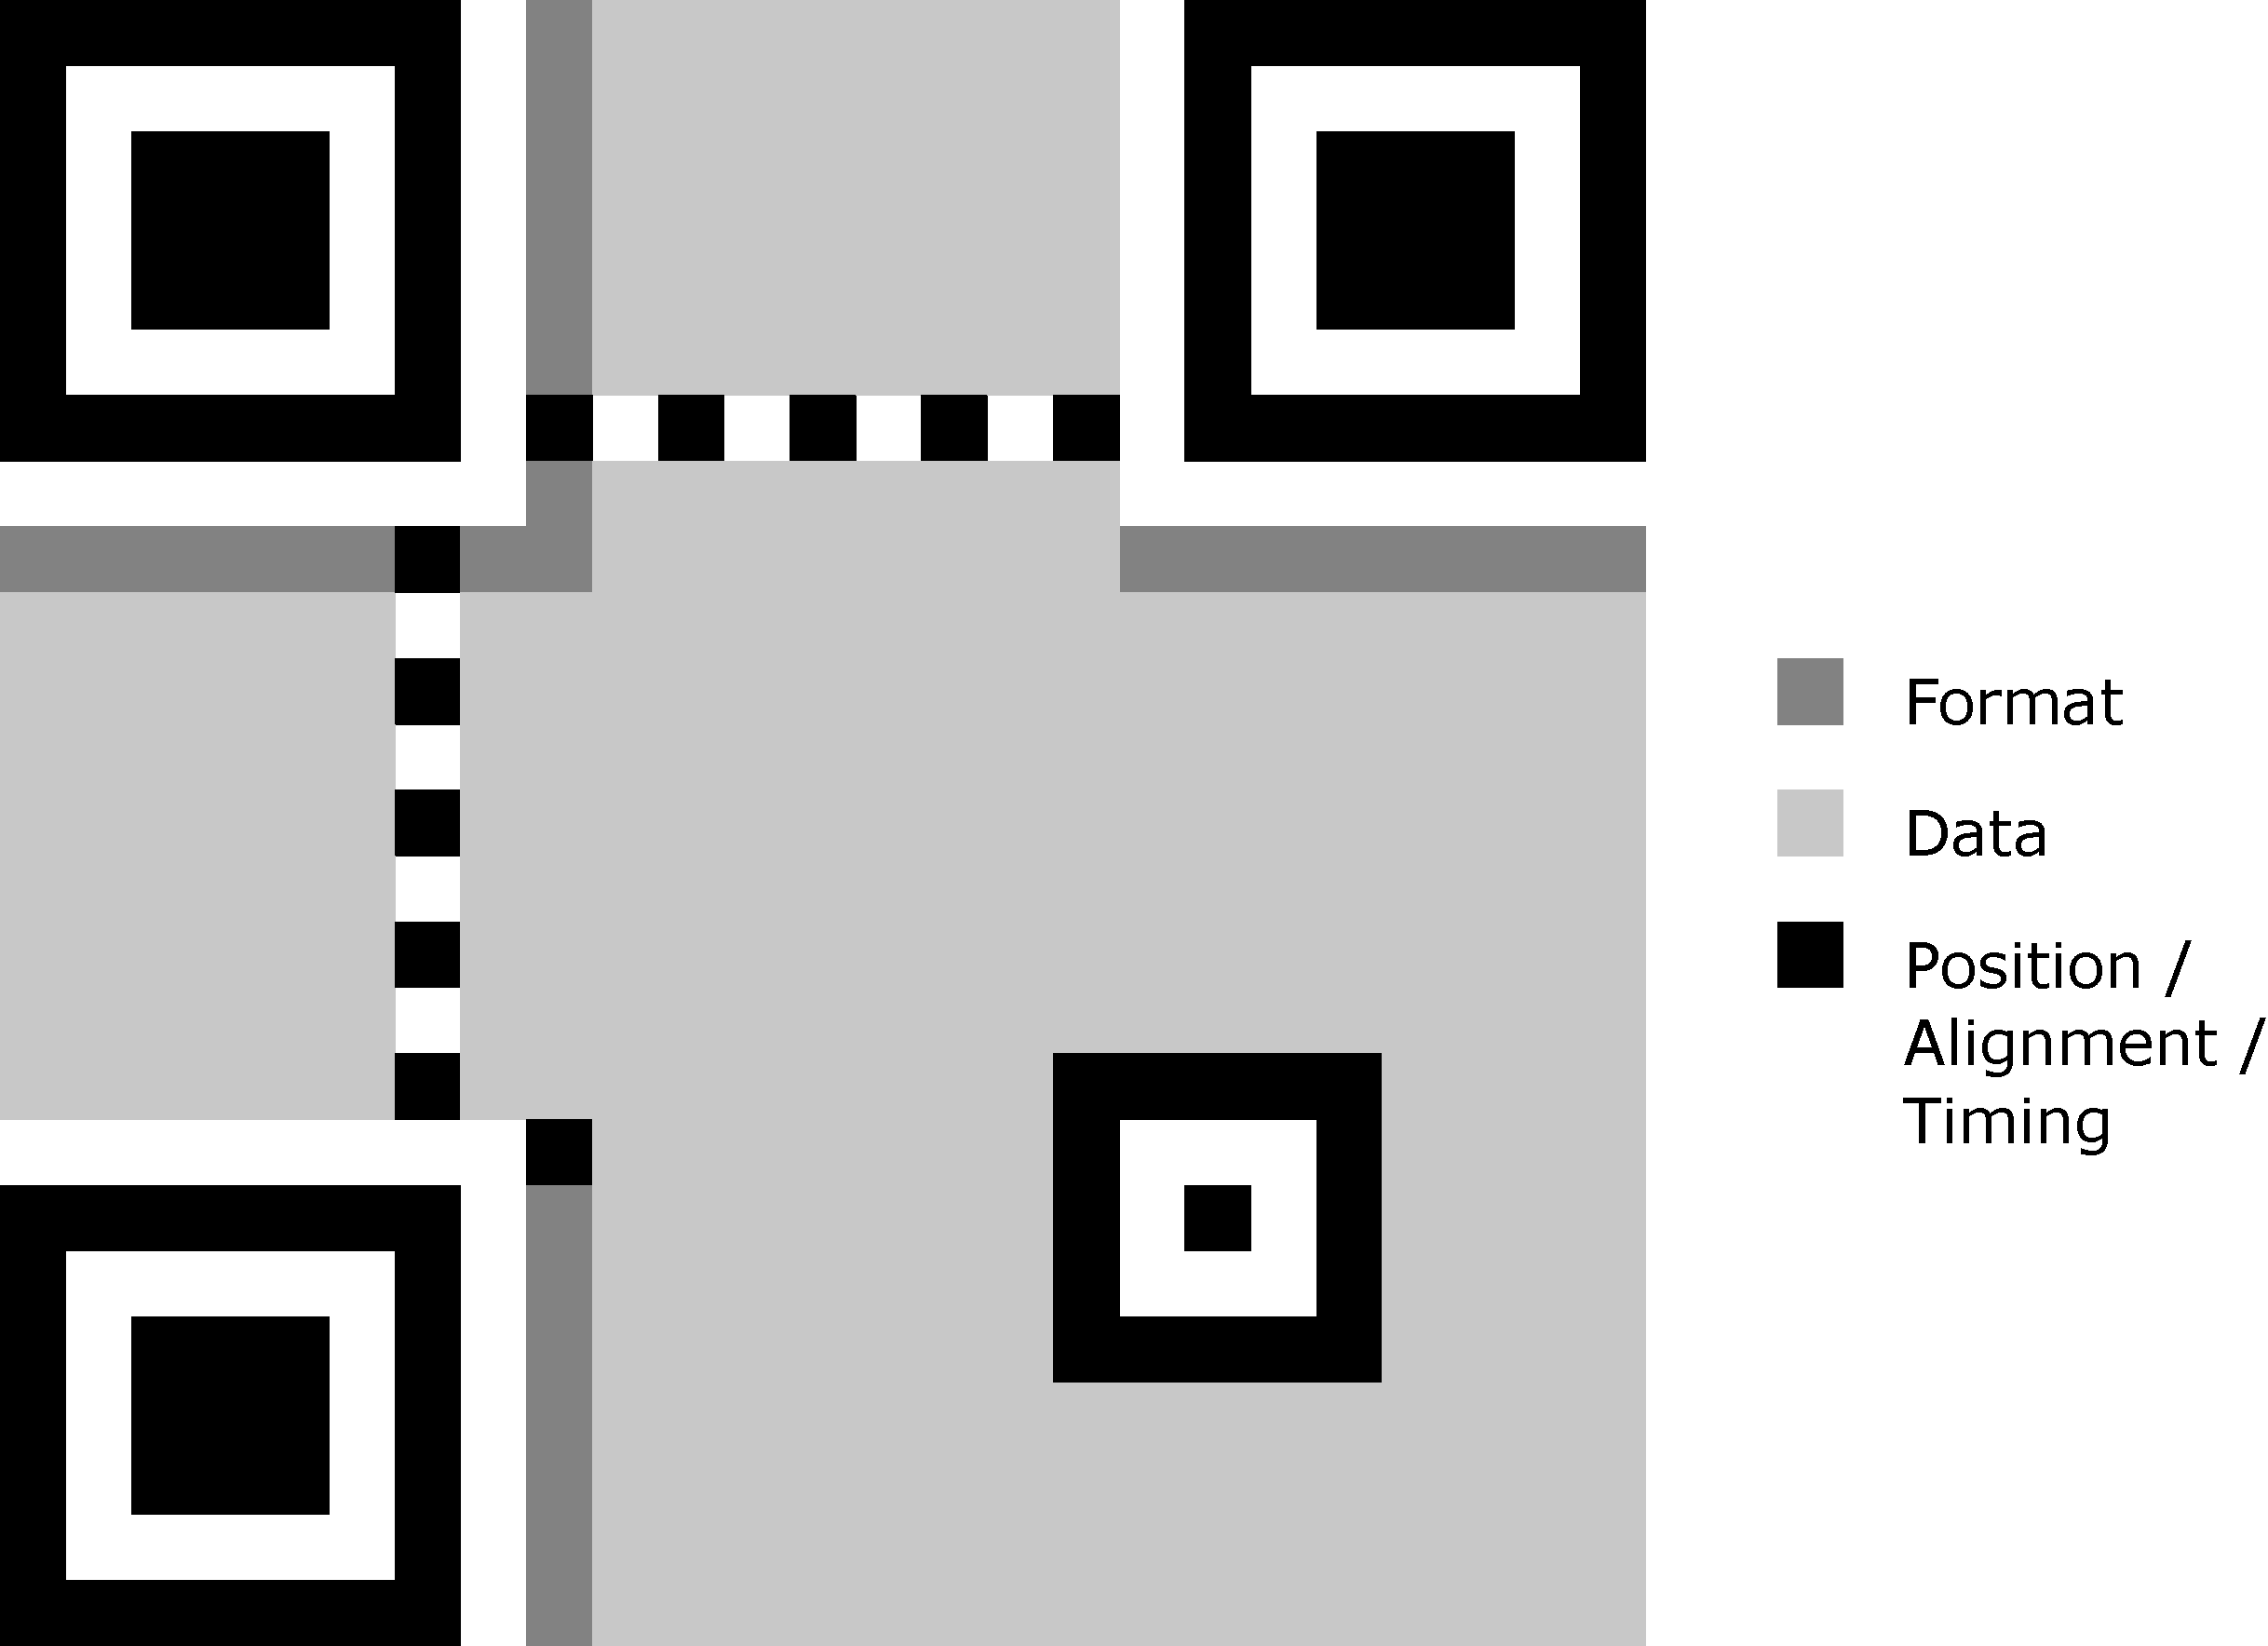
\includegraphics[width=80mm]{images/qrcodeMall}
		\caption{The standardised fields of a QR code~\cite{qrCodeWiki}.}
		\label{qrcodeMall}
	\end{figure}
	 
A QR code can be used to encode information, originally written with alphabetic characters, japanese symbols (Kanji) or numeric characters~\cite{qrCodeVersion}. With the help of a QR code information which would otherwise have taken up a large space can now be easily fitted in smaller areas.

\subsubsection{Decoding}
Decoding a QR code is a fairly straight forward process which, although time consuming, can be done by hand, as described in several guides around the Internet~\cite{qrcodeDecoding2, qrcodeDecoding, qrcodeDecoding3}. A QR code may be divided in to three standardised fields, which help QR code scanners to identify and decode QR codes. The three fields can be seen in Figue~\ref{qrcodeMall}. The position, alignment and timing fields are used to identify and position the QR code correctly as a QR code may be scanned from any direction. In order to decode a QR code the three main position fields residing in three of the QR code's corners must be positioned as seen in Figure~\ref{qrcodeExample}.

The next step is to identify the mask used on the data field in the QR code. The mask is used to remove any large, empty or filled, areas within the data field which might make the decoding process more difficult for QR code scanners. The mask field is a part of the format field, seen in Figure~\ref{qrcodeMall}. The format field holds information about error correction, as well as which mask has been used on the data field. The mask is found among the first five bits in the format field. The first two bits of the first five bits of the format field contain information regarding the amount of error correction data the QR code contains, and the other three contain information on which mask has been used.

	\begin{figure}[H]%ht!]
		\centering
		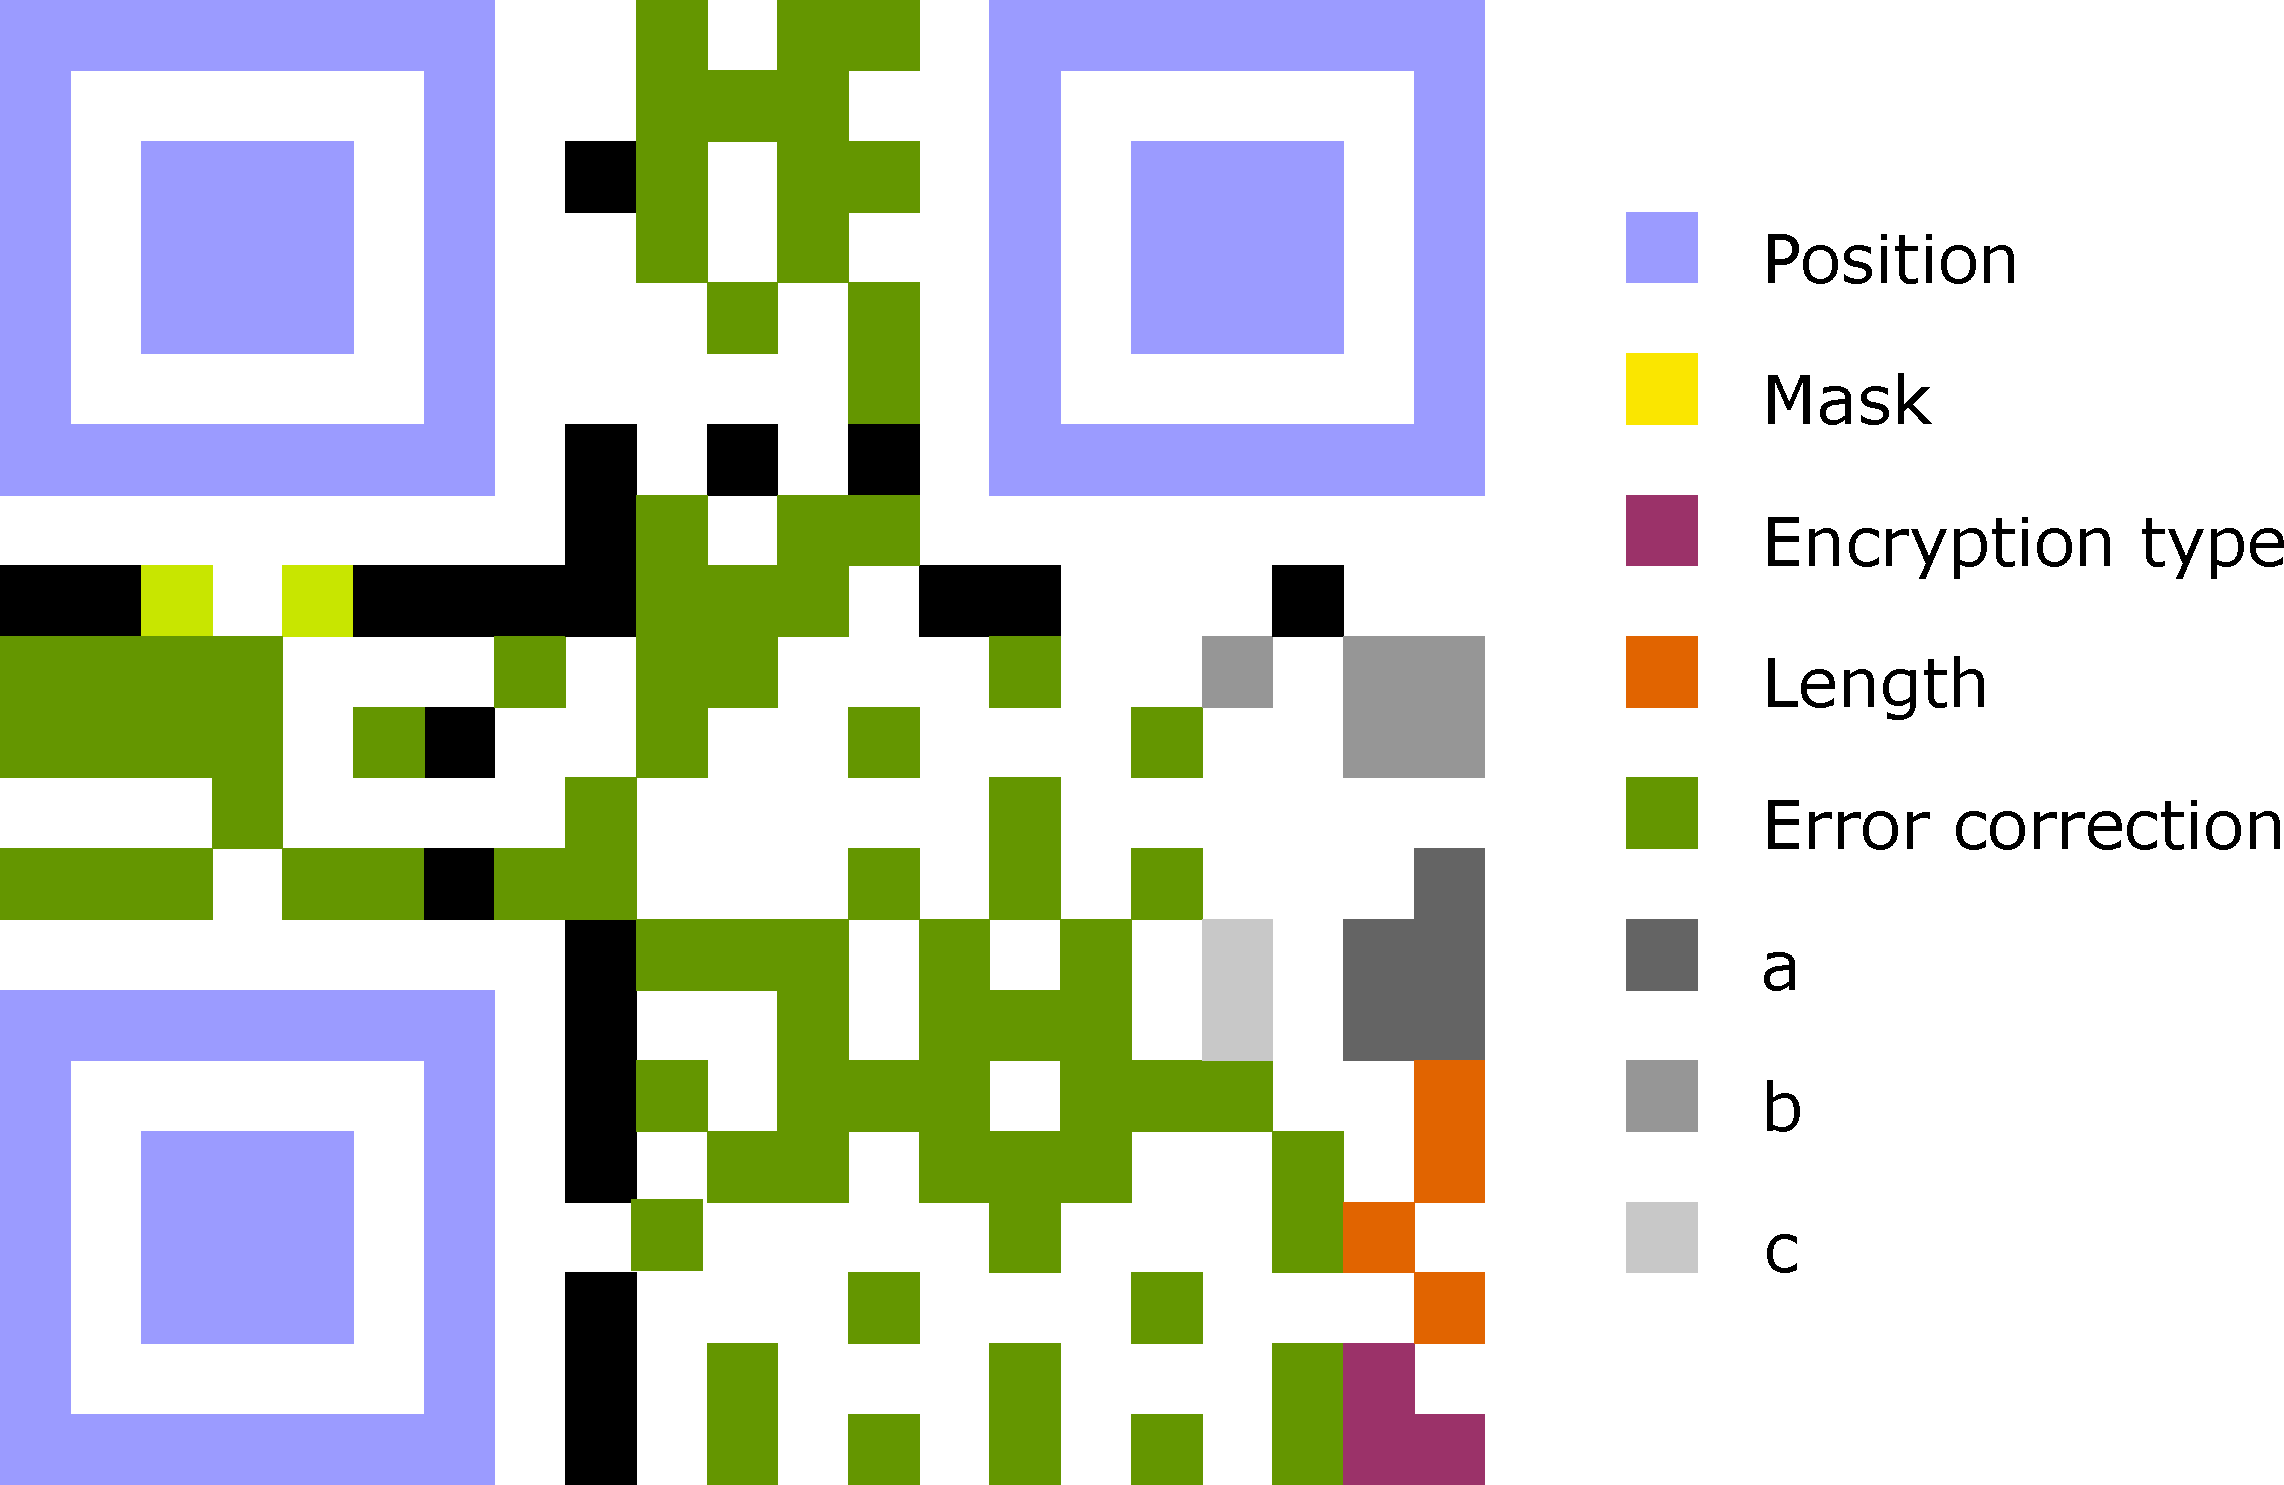
\includegraphics[width=100mm]{images/qrcodeexample}
		\caption{A QR code example, encoded with the string "abc".}
		\label{qrcodeExample}
	\end{figure}

In Figure~\ref{qrcodeExample} the mask field has the value of 101, seen more clearly in Figure~\ref{qrcodeExampleStep3}. Filled blocks should be interpreted as a 1 and empty blocks should be interpreted as a 0. However, the mask field is always XOR:d with 101 prior to being printed in the QR code and must as such be XOR:d back to the original mask value. In the case of Figure~\ref{qrcodeExample} the original mask value is calculated as follows:

\begin{center}
	101~XOR~101 = 000
\end{center}

	\begin{figure}[H]%ht!]
		\centering
		\fbox{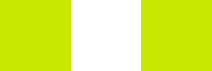
\includegraphics[width=30mm]{images/qrcodeexampleStep3}}
		\caption{Mask pattern encoded as 101.}
		\label{qrcodeExampleStep3}
	\end{figure}

There are eight different mask patterns in total, each represented by a unique bit string. The mask pattern represented by 000 can be seen in Figure~\ref{qrcodemaskpattern}, while the rest of the mask patterns may be found here~\cite{qrcodeMaskPatterns}. The mask used in Figure~\ref{qrcodeExample} means that all bits should be flipped if the following formula is true:

\begin{center}
	\((i+j)~mod~2=0\), 

	where i and j represents the indexes of the specific block, horizontally and vertically respectively~\cite{qrcodeMaskPatterns}.
\end{center}

	\begin{figure}[H]%ht!]
		\centering
		\fbox{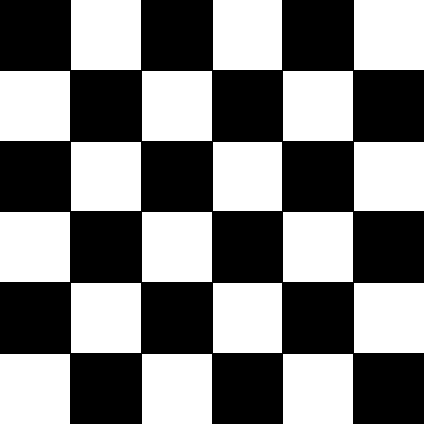
\includegraphics[width=40mm]{images/qrcodemaskpattern}}
		\caption{Mask pattern represented by the bit string 000~\cite{qrcodeMaskPatterns}.}
		\label{qrcodemaskpattern}
	\end{figure}
	
Having decoded the mask pattern the next step is to decode the data area. The data area always contains a header, containing information on the encryption type as well as data length. The blocks containing the encryption type is always the size of four blocks, and always located in the lower right corner, as seen in Figure~\ref{qrcodeExample}. The number of blocks used for the data length may vary between eight and ten blocks depending on the encryption type.

As such the first step in decoding the data area is to decode the encryption type. The information in the data area is to be read from the lower right and upwards, in a zig-zag pattern, with a width of two blocks. When reaching the top the zig-zag pattern continues, although downwards. See Figure~\ref{qrcodezigzag} for a better understanding of the zig-zag pattern. The start point is always in the lower right corner since the encryption type must be decoded first.

	\begin{figure}[H]%ht!]
		\centering
		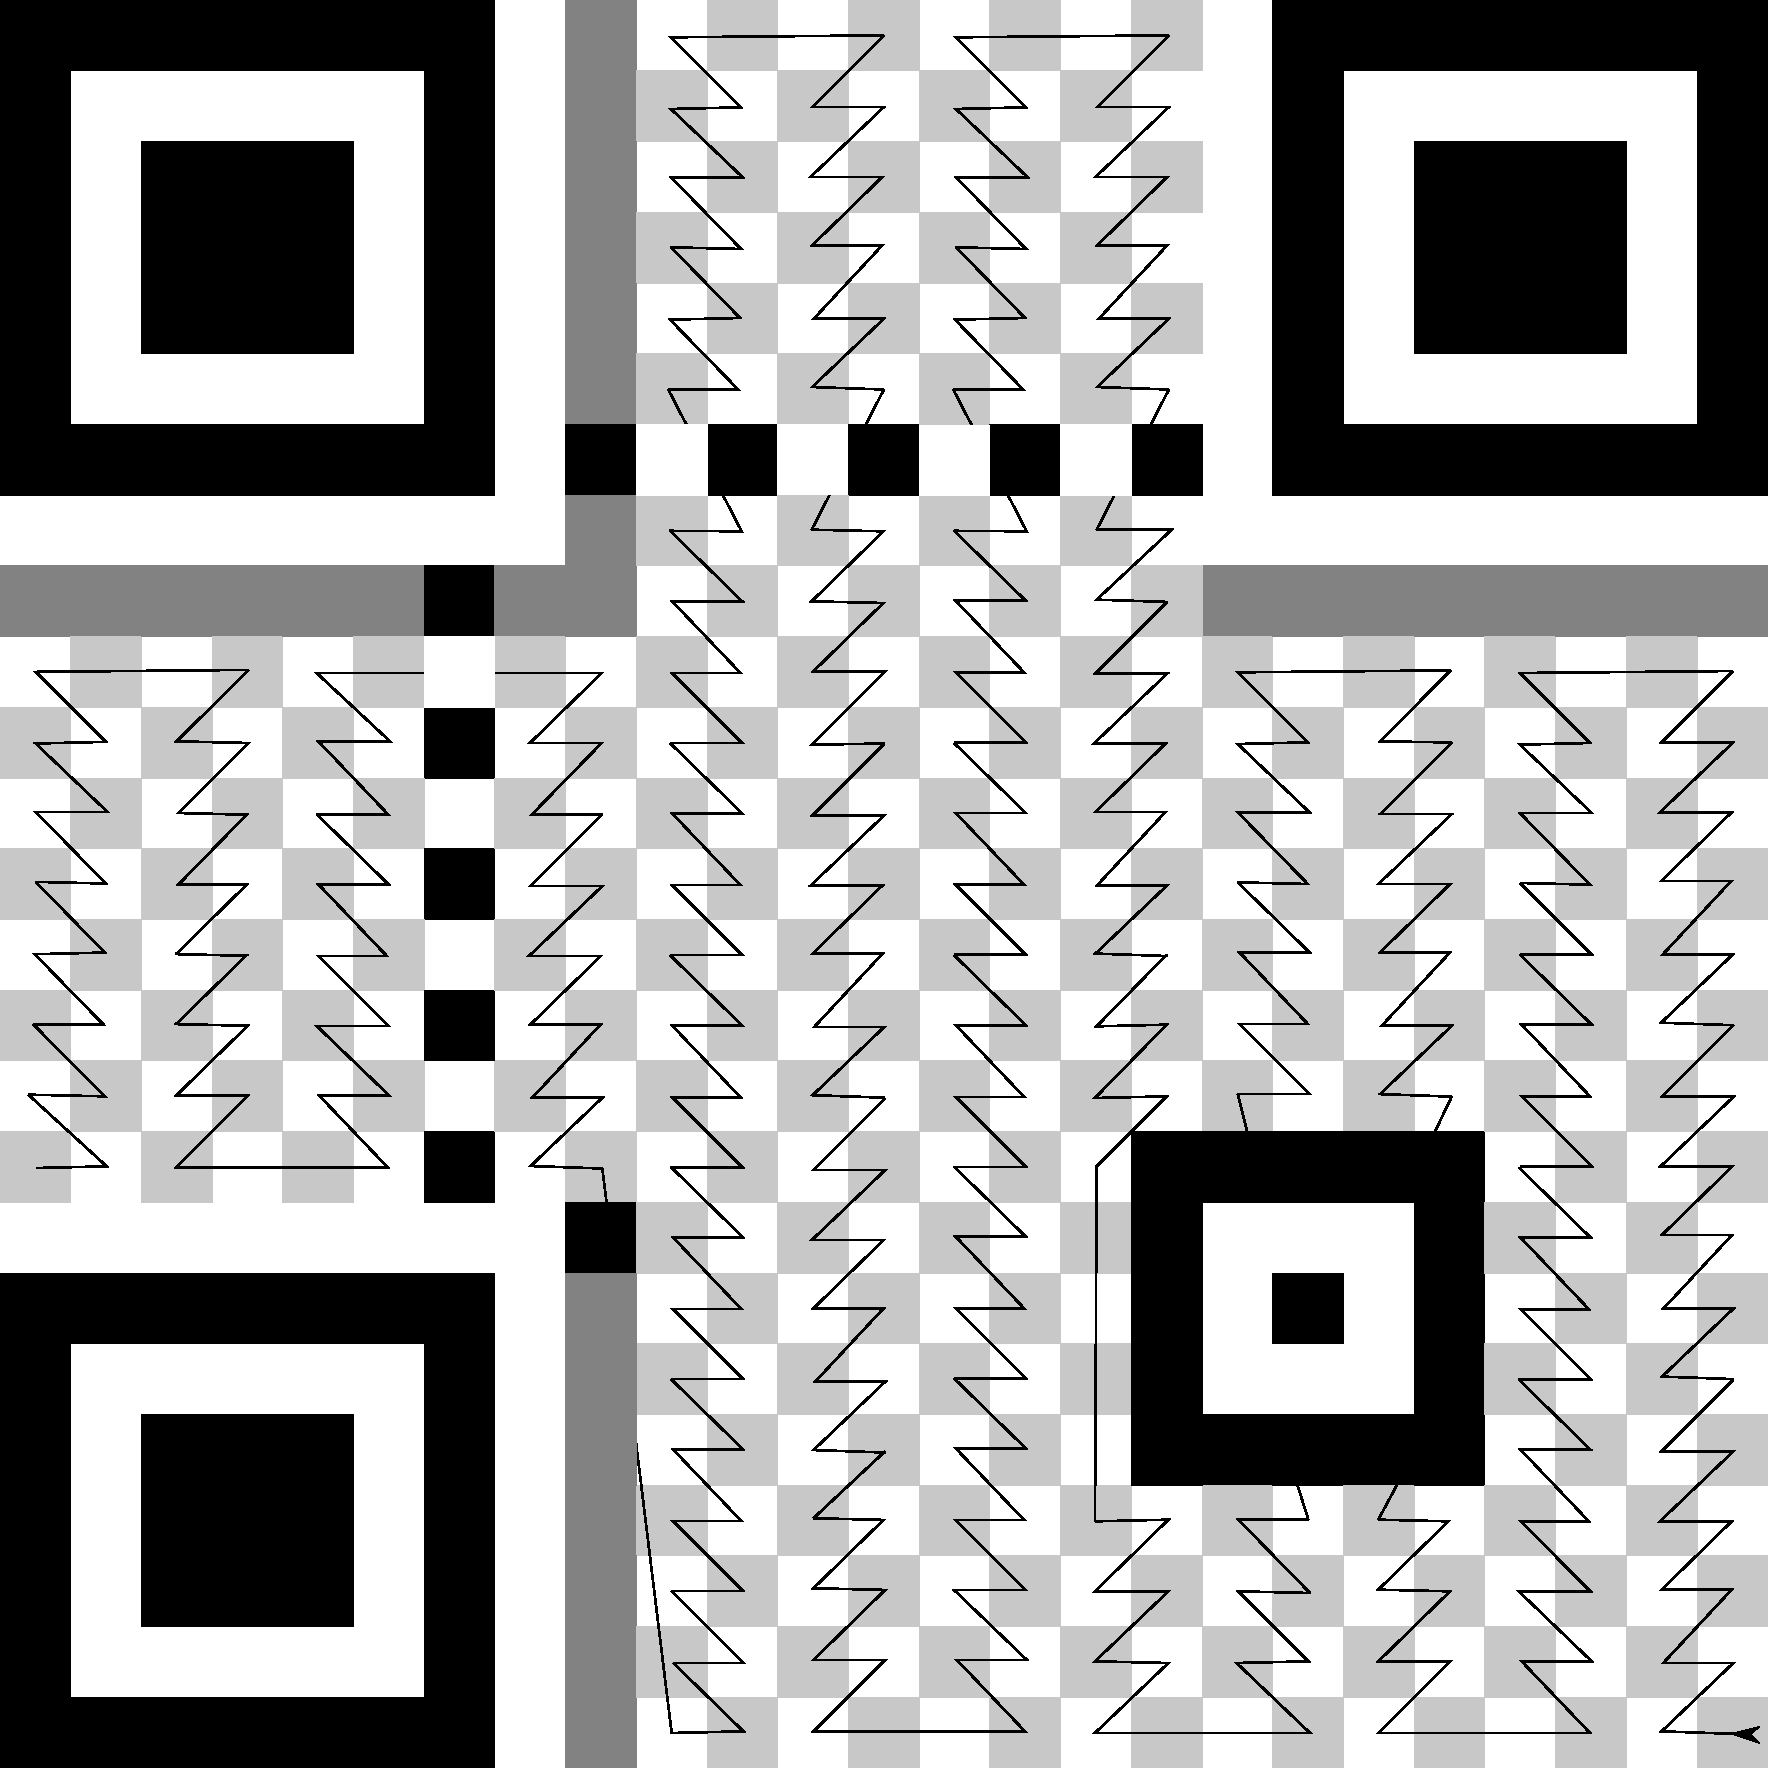
\includegraphics[width=100mm]{images/qrcodezigzag}
		\caption{The zig-zag pattern used when decoding a QR code.}
		\label{qrcodezigzag}
	\end{figure}

Using the zig-zag pattern the encryption type bit string in Figure~\ref{qrcodeExample} can be found to be 1101, seen more clearly in Figure~\ref{qrcodeExampleStep4}. However, the encryption type is a part of the data section and as such must be unmasked. Using the mask formula gives the following results:

\begin{center}

\((20+20)~mod~2=40~mod~2=0\)

\((20+19)~mod~2=39~mod~2=1\)

\((19+20)~mod~2=39~mod~2=1\)

\((19+19)~mod~2=38~mod~2=0\)

\end{center}

	\begin{figure}[H]%ht!]
		\centering
		\fbox{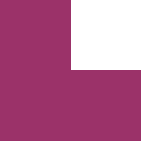
\includegraphics[width=15mm]{images/qrcodeexampleStep4}}
		\caption{Encryption type encoded as 1101.}
		\label{qrcodeExampleStep4}
	\end{figure}

As such the blocks at position (i, j) = (19, 19), and (i, j) = (20, 20) must be flipped. The ``flipping'' process may be done by XOR:ing the massked encryption type bit string with a bi string representing the bits that must be ``flipped'', putting ones at the positions where the corresponding bit in the masked encryption type bit string must be flipped, and zeroes at the position where the corresponding bit does not need to be flipped. The masked encryption type bit string, 1101, must as such be XOR:d with 1001, as follows:

\begin{center}
\(1101~XOR~1001=0100\)
\end{center}

There are several encryption types used in QR codes, however the most common ones are the following (represented by the following bit strings):

\begin{itemize}
	\item 0001 Numeric
	\item 0010 Alphanumeric
	\item 0100 8-Bit Byte
\end{itemize}

The encryption type used in Figure~\ref{qrcodeExample} is as such of encryption type 8-bit Byte.

After having decoded the encryption type the next step is to decode the length. The encoded length is the length of the message encoded in the QR code. Since the message encoded in the QR code may not cover the entire data section of the QR code (the rest is made up of error correction information) the length of the message is necessary in order to know when the message ends. Since the encryption type used in Figure~\ref{qrcodeExample} is an 8-bit Byte the size of each field that follows is eight bits in size.

The length field in Figure~\ref{qrcodeExample}, seen also in FIgure~\ref{qrcodeExampleStep5}, is the following bit string: 10011010. However, the length field is a part of the data section and must as such be unmasked in order for the original length value to be obtained.

	\begin{figure}[H]%ht!]
		\centering
		\fbox{
\includegraphics[width=15mm]{images/qrcodeexampleStep5}}
		\caption{The message length encoded as 10011010.}
		\label{qrcodeExampleStep5}
	\end{figure}

\begin{center}

\((18+20)~mod~2=38~mod~2=0\)

\((18+19)~mod~2=37~mod~2=1\)

\((17+20)~mod~2=37~mod~2=1\)

\((17+19)~mod~2=36~mod~2=0\)

\((16+20)~mod~2=36~mod~2=0\) 

\((16+19)~mod~2=35~mod~2=1\)

\((15+20)~mod~2=35~mod~2=1\)

\((15+19)~mod~2=34~mod~2=0\)

\end{center}

The encryption type bit string must as such be XOR:d with 10011001, as follows:

\begin{center}
\(10011010~XOR~10011001=00000011=3\)
\end{center}

The message in Figure~\ref{qrcodeExample} is as such of length 3.

Finally, the data is decoded. The first 8-bit Byte, seen in Figure~\ref{qrcodeExampleStep6}, gives the following bit string: 11111000. However, being a part of the data section, the bit string must be unmasked, as follows:

\begin{center}

\((14+20)~mod~2=34~mod~2=0\)

\((14+19)~mod~2=33~mod~2=1\)

\((13+20)~mod~2=33~mod~2=1\)

\((13+19)~mod~2=32~mod~2=0\)

\((12+20)~mod~2=32~mod~2=0\) 

\((12+19)~mod~2=31~mod~2=1\)

\((11+20)~mod~2=31~mod~2=1\)

\((11+19)~mod~2=30~mod~2=0\)

\end{center}

The first 8-bit Byte bit string must as such be XOR:d with 10011001.

\begin{center}
\(11111000~XOR~10011001 = 01100001 = 64 + 32 + 1 = 97\)
\end{center}

	\begin{figure}[H]%ht!]
		\centering
		\fbox{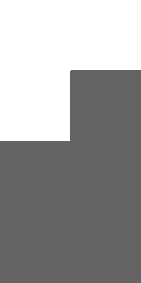
\includegraphics[width=15mm]{images/qrcodeexampleStep6}}
		\caption{The first 8-bit Byte encoded as 11111000.}
		\label{qrcodeExampleStep6}
	\end{figure}

The second 8-bit Byte, seen in Figure~\ref{qrcodeExampleStep7}, reaches the top of the data section and as such the last four bits must be read horizontally to the left, as described in Figure~\ref{qrcodezigzag}. Doing so gives the following bit string: 11110100. Again, the bit string must be unmasked.

\begin{center}

\((10+20)~mod~2=30~mod~2=0\)

\((10+19)~mod~2=29~mod~2=1\)

\((9+20)~mod~2=29~mod~2=1\)

\((9+19)~mod~2=28~mod~2=0\)

\((9+18)~mod~2=27~mod~2=1\) 

\((9+17)~mod~2=26~mod~2=0\)

\((10+18)~mod~2=28~mod~2=0\)

\((10+17)~mod~2=27~mod~2=1\)

\end{center}

The second 8-bit Byte bit string must as such be XOR:d with 10010110.

\begin{center}
\(11110100~XOR~10010110 = 01100010 = 64 + 32 + 2 = 98\)
\end{center}

	\begin{figure}[H]%ht!]
		\centering
		\fbox{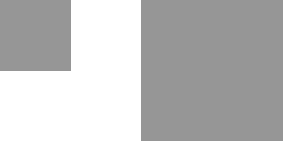
\includegraphics[width=30mm]{images/qrcodeexampleStep7}}
		\caption{The second 8-bit Byte encoded as 11110100.}
		\label{qrcodeExampleStep7}
	\end{figure}

The third, and final 8-bit Byte, seen in Figure~\ref{qrcodeExampleStep8}, to be decoded is read downwards as described in Figure~\ref{qrcodezigzag}, giving the following bit string: 00000101. The bit string must be unmasked:

\begin{center}

\((11+18)~mod~2=29~mod~2=1\)

\((11+17)~mod~2=28~mod~2=0\)

\((12+18)~mod~2=30~mod~2=0\)

\((12+17)~mod~2=29~mod~2=1\)

\((13+18)~mod~2=31~mod~2=1\) 

\((13+17)~mod~2=30~mod~2=0\)

\((14+18)~mod~2=32~mod~2=0\)

\((14+17)~mod~2=31~mod~2=1\)

\end{center}

The third 8-bit Byte bit string must as such be XOR:d with 01100110.

\begin{center}
\(00000101~XOR~01100110 = 01100011 = 64 + 32 + 2 + 1 = 99\)
\end{center}

	\begin{figure}[H]%ht!]
		\centering
		\fbox{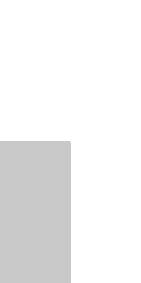
\includegraphics[width=15mm]{images/qrcodeexampleStep8}}
		\caption{The third 8-bit Byte encoded as 00000101.}
		\label{qrcodeExampleStep8}
	\end{figure}

Since the message length was found to be of size 3 all parts of the message in Figure~\ref{qrcodeExample} have been found. The rest of the data section contains information regarding error correction, used in case the QR code was somehow damaged.

The message in Figure~\ref{qrcodeExample} has been decoded as 97, 98 and 99. Converting there numbers using an ASCII table gives the following result: a, b and c~\cite{asciitable}. The encoded message in Figure~\ref{qrcodeExample} has as such been decoded to ``abc'', which is correct and may be checked by scanning Figure~\ref{qrcodeExample} using a QR code scanner.

Although the decoding of a QR code may seem like an extensive process, the process may be divided in to the following five parts:

\begin{enumerate}
	\item Aligning the position
	\item Finding the mask used on the data section
	\item Unmasking the encryption type
	\item Unmasking the length of the encoded message
	\item Unmasking the message
\end{enumerate}

Although time consuming, decoding information from a QR code by hand is possible and follows the same steps as a QR code scanner.